% 卒業研究前刷テンプレート
% lualatex用

\RequirePackage{plautopatch}

\documentclass[a4paper,10pt]{ltjsarticle}
\usepackage{luatexja}
\usepackage{enumitem} % リストカスタマイズ用
\usepackage{geometry}
\usepackage{multicol}
\usepackage{amsmath}
\usepackage{titlesec}
\usepackage{indentfirst}
\usepackage{graphicx}
\usepackage{here}
\usepackage{fancyvrb}

\geometry{
top=20mm,
bottom=20mm,
left=20mm,
right=20mm
}\setlength{\columnsep}{7.5mm}

\linespread{0.8}

\titleformat{\section}{\normalsize}{\thesection}{1em}{}
\titleformat{\subsection}{\normalsize}{\thesubsection}{1em}{}
\titlespacing*{\section}{0pt}{1.0ex plus 1ex minus .2ex}{1ex plus .2ex}
\titlespacing*{\subsection}{0pt}{1.0ex plus 1ex minus .2ex}{0.5ex plus .2ex}
\DefineVerbatimEnvironment{smallverbatim}{Verbatim}{fontsize=\footnotesize}

\makeatletter
 \def\@maketitle{
 \begin{flushright}
 {\large \@date}
 \end{flushright}
 \begin{center}
 {\LARGE \@title \par}
 \end{center}
 \begin{flushright}
 {\@author}
 \end{flushright}
 \par\vskip 1.5em
 }
\makeatother

\title{\huge ドローンネットワークにおける直線中継伝送の\\アクセス制御方式の検討\\
\Large A Study on Access Control Schemes for Rectilinear Relay Transmission \\in Drone Networks
}

\author{
T5-25 \:中村 優\\
指導教員 \: 設樂 勇
}

\date{}

\begin{document}
% タイトル部分は1カラムで表示
\twocolumn[
\maketitle
]

% ---------
% 本文開始
% ---------
\section{はじめに}
ドローンを用いたネットワークにおいて,オーバーリーチの問題を解決するために送信信号の届く中継局まで一度に中継するCTR(Cooperation Through Relay)方式[1]が提案されている. 本稿では,提案手法において干渉/誤りが生じた際のスループット特性を従来方式と比較し評価する.
\section{従来方式の概要}
図1に従来方式である概要を示す.従来の中継伝送では1ホップずつ中継するが,自由空間では,伝搬損失が少ないため送信信号が中継先のドローン(図1\#3)より遠くのドローン(図1\#4)に到達することで干渉が生じる.そのため,従来方式はオーバーリーチ干渉によってパケットの再送が起こりチャネルの利用効率が低下する.また,従来方式で干渉が生じ,再送を行う際には,フォールバック制御により伝送レートを下げることでSNR(Signal to Noise Ratio)が低くてもパケットを受信できるようにしているが,伝送レートの低下に伴って送信時間や再送によるオーバヘッドが増加してしまう課題がある.%伝送レート 受信感度 SN比 本番では説明

\begin{figure}[H]
  \centering
  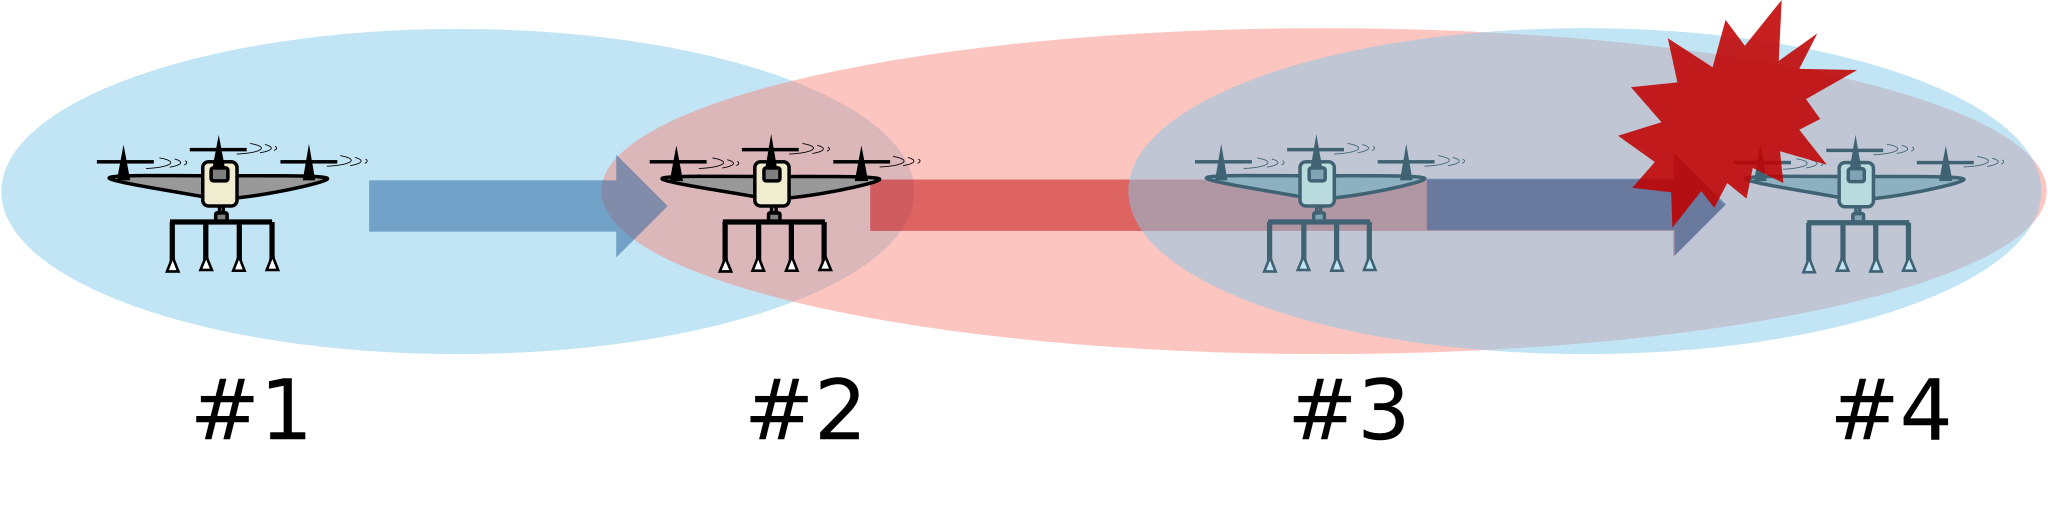
\includegraphics[width=\linewidth]{cenventional_topology.pdf} % 図のファイル名を指定
  \caption{従来の方式の概要}
  \label{fig:従来の方式のトポロジー} % 参照用ラベル
\end{figure}

\section{CTR方式の概要}
オーバリーチ干渉は送信信号が中継局のドローンを超えて他のドローンに干渉することで発生する.そこでCTR方式では直線状に存在する中継局が協調することによってオーバリーチ干渉の問題を解決する.
図2に示すCTR方式は,送信信号の届く範囲の最終中継局(図 1\#4)まで一度に信号を送信し,通信経路の中継局(図1\#3)も協調してパケットを受信する.最終中継局がパケットを正常に受信した場合は,以後,同様の手順で中継する.最終中継局がパケットの受信に失敗した場合は,直線経路の中継局\#3が\#4の代わりに次の中継局へパケットを中継する.そのため従来方式ではオーバーリーチ干渉が生じる環境でもCTR方式ではオーバーリーチ干渉が減り中継ホップ数も減るので中継オーバヘッドも削減することができる.%オーバーリーチ干渉の影響を減らす→オーバーリーチ干渉が生じる環境でも...
\begin{figure}[H]
  \centering
  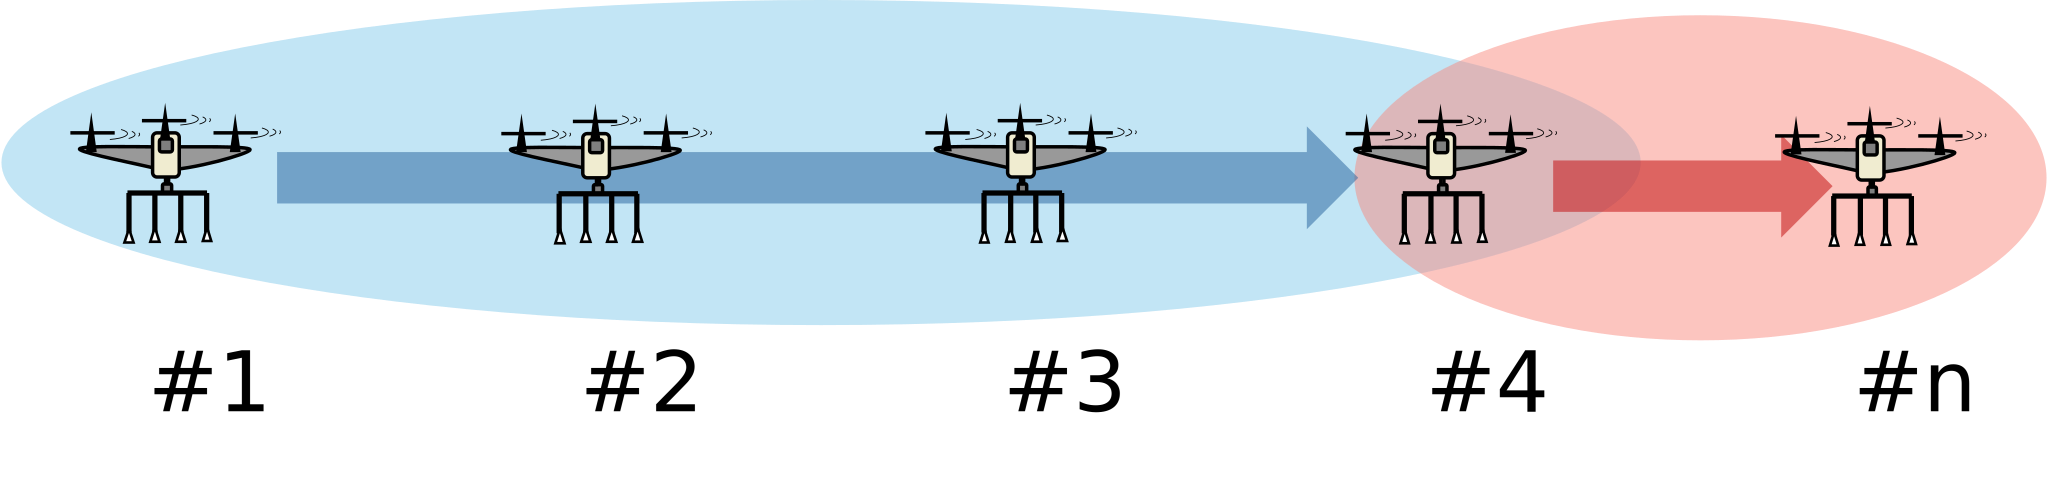
\includegraphics[width=\linewidth]{CTR_topology.pdf} % 図のファイル名を指定
  \caption{CTR方式の概要}
  \label{fig:CTR方式のトポロジー} % 参照用ラベル
\end{figure}
図3にCTR方式の詳細なアクセス制御手順を示す.通常のCSMA/CA(Carrier Sense Multiple Access/Collision Avoidance)と同様に送信局はランダム時間のBackoffの後,ACK(ACKnowledgement)duration
時間が記述されたパケットを送信する.パケットを受信した中継局は送信局に対してACK duration時間後にACKを返信する.
このとき,ACKを受信した経路上の中継局はACKの送信待ちをキャンセルする.最終中継局(図2\#4)がパケットを受信できない場合は\#3が送信局の\#1にACKを送信し,\#4の代わりに中継する.
ACK duration はスロットタイム区切りとなっており,最終受信中継局が最もACK durationが短く,送信局に近づくにつれて1ずつスロットタイム増加していく.
したがって,このCTR方式は信号が届く最大の範囲を推定する必要がある.そのため,送信電力の制御に加え各端末のSNRの受信電力閾値から自律的に判断し中継制御を行う.

\begin{figure}[H]
  \centering
  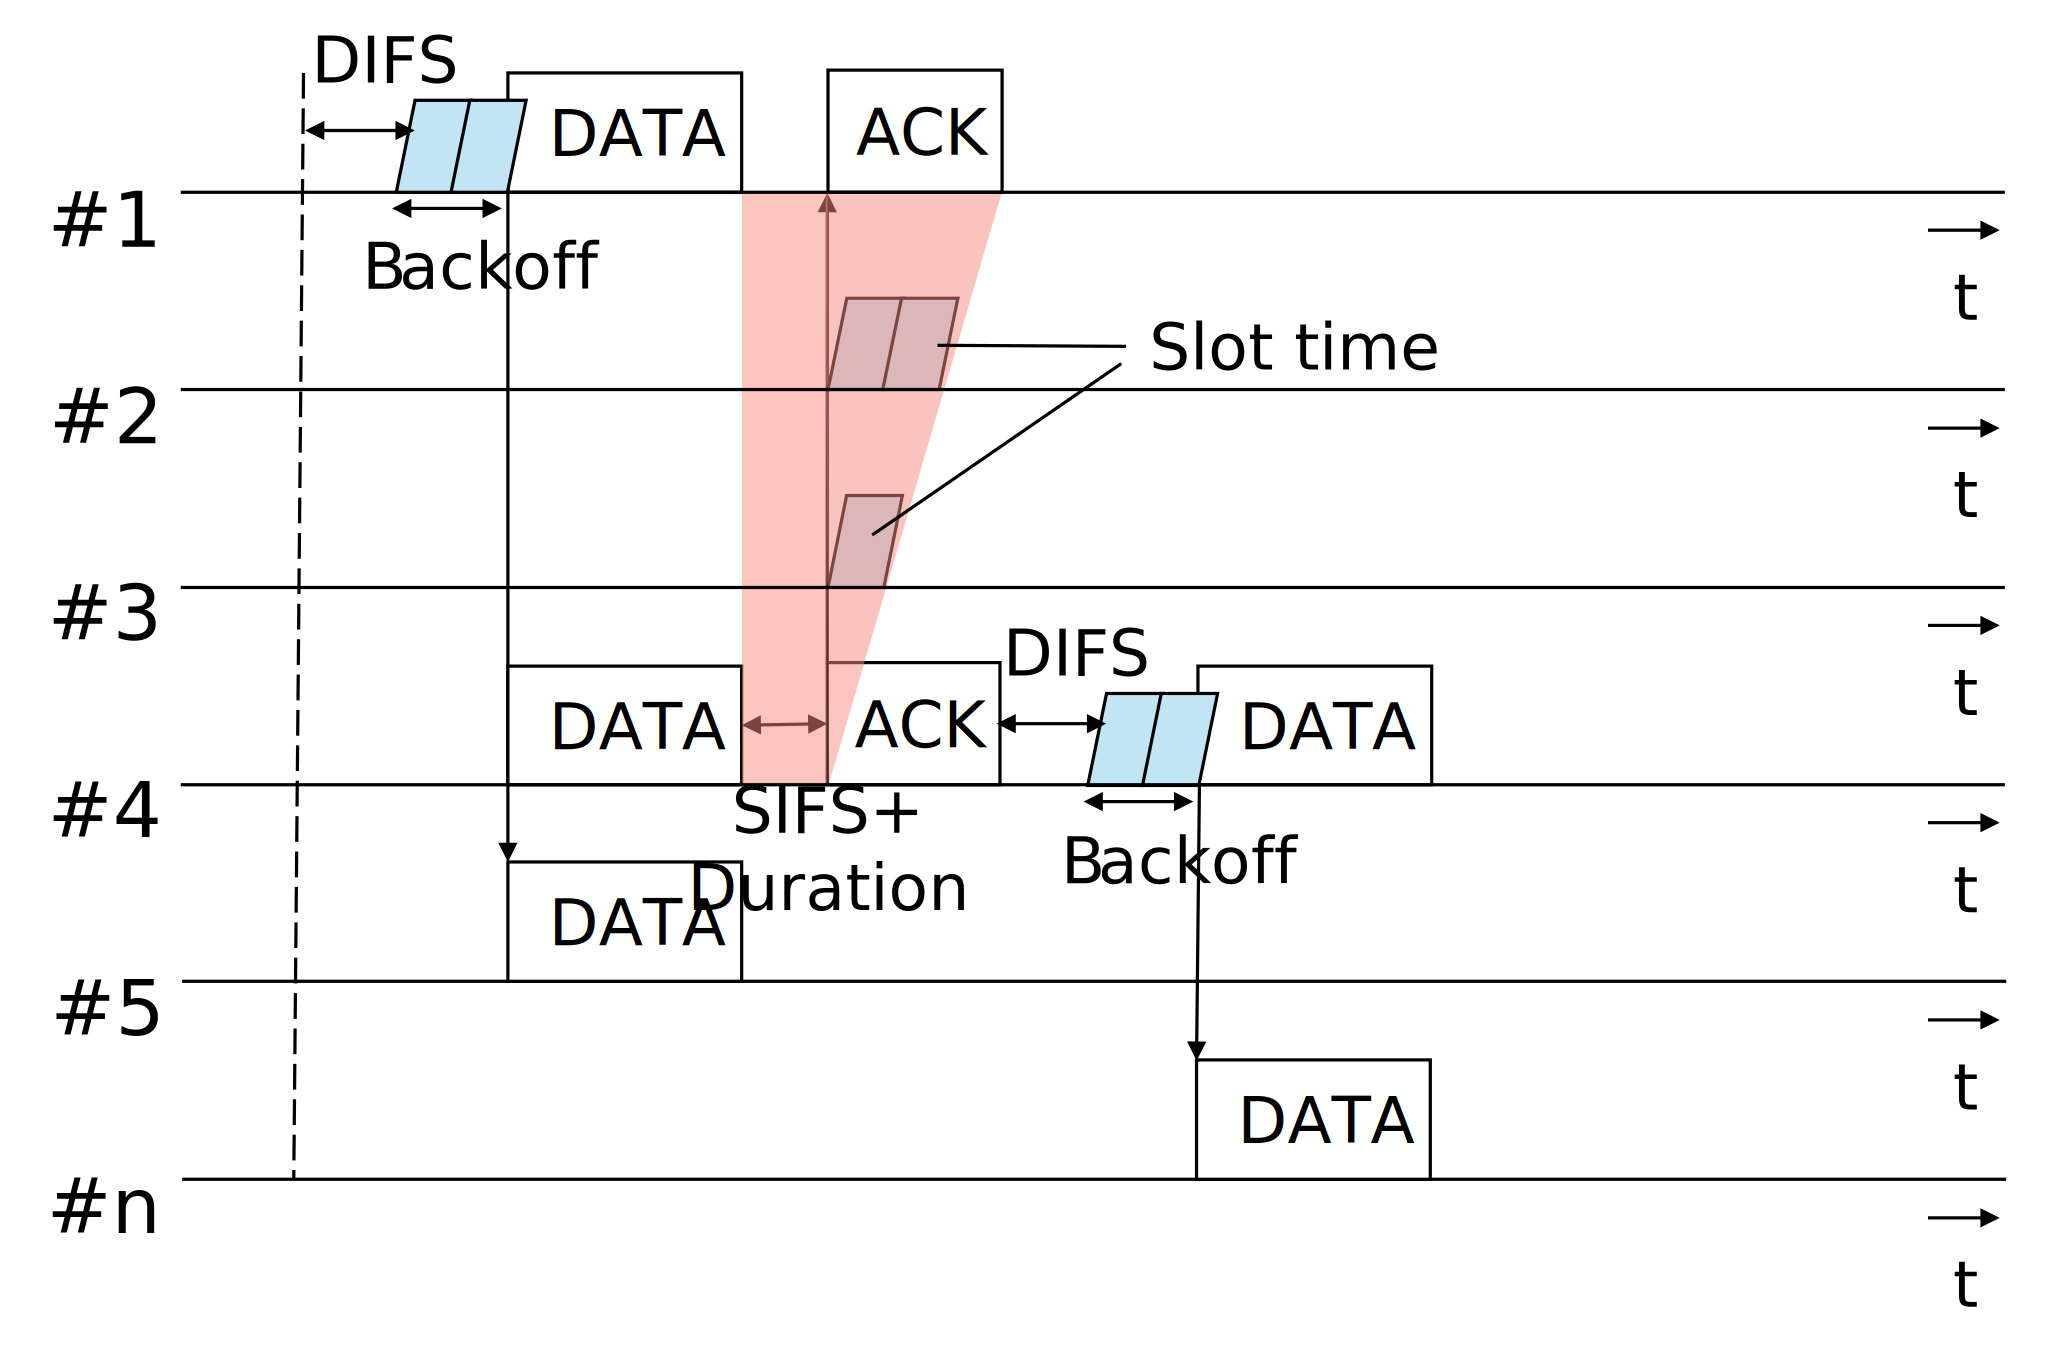
\includegraphics[width=\linewidth]{CTR_accsess.pdf} % 図のファイル名を指定
  \caption{CTR方式のアクセス制御}
  \label{fig:CTR方式のアクセス制御} % 参照用ラベル
\end{figure}
\section{CTR方式の評価}
\subsection{誤りが無い条件でのCTR方式の評価}
CTR方式の特徴である中継局をスルーすることによるスループットの向上を下記の条件で従来方式と比較する.%中継局スルーすることによるスループットの向上を従来の方式と比べて下記の条件で...
中継の総伝送距離は1000mとし,50m間隔で直線状に20台のドローンを配置した.アンテナの送受信利得は0dBi,送信電力は10dBmとした.周波数は2.4GHz,伝送レートはIEEE 802.11gを参考にし,伝搬損失は自由空間伝搬損失とした.
評価内容は従来の1ホップ中継(54Mbps) と中継局を2台スルー(24Mbps) した場合,
および中継局を3台スルー(18Mbps) した場合におけるスループット特性を確認する.括弧内は使用可能な最も高い伝送レートである.これは受信電力よりIEEE 802.11gのMCS (Modulation and Coding Scheme) indexから選択する.
図4にCTR方式のスループット特性を示す.従来の1ホップ中継と比べてCTR方式で中継局を3台スルーした条件では約2倍のスループットが得られた.
ドローンをスルーする場合は,通信距離が長くなり使用可能な伝送レートが低下するが、アクセス制御やプリアンブル等のオーバヘッドとのトレードオフになる.その結果,ネットワーク全体の通信効率において,中継局を3台スルーする条件が最も高くなることが分かる.
.
\begin{figure}[H]
  \centering
  \includegraphics[width=\linewidth]{throughtput_vs_placement_50m_max_distance_3.pdf} % 図のファイル名を指定
  \caption{CTR方式のスループット特性}
  \label{fig:throughput_through} % 参照用ラベル
\end{figure}
\subsection{誤りを生じる条件でのCTR方式の評価}
CTR方式のもう一つの特徴である中継時に誤りが生じたときに経路上の中継局が代替して受信することによる効果を下記の条件で従来方式と比較する.
条件は4.1と同じ条件を用いる.また4.1より中継局を3台スルー(18Mbps)したとき最もスループットが高いことから伝送レートは18Mbpsとする.従来方式では再送時のフォールバック制御により伝送レートを一つ下の12Mbpsで再送は必ず成功するとする.この時パケットの誤り率を0\%から100\%まで変化させたときの1000m地点での最終的なスループット特性をを従来の方式とCTR方式のスループットで比較した.
\\ 図5に誤り率が変化したときスループットを示す.従来方式では誤り率が増加するにつれスループットが一定の割合で減少しているが、CTR方式ではスループットが緩やかに減少する部分があることが分かる.これはパケットの送信回数が関係していると考える.図6には誤り率に対しての1000m地点に辿り着くまでの平均送信回数を示す.図6より従来方式の送信回数は誤り率に対して線形的に変化しているが,CTR方式の送信回数は非線形的に増加している.これは,CTR方式で誤りが生じた際に,一つ前の中継局が通信を代替するからで,その結果、パケットの誤り率が変化しても送信回数の増加は緩やかに抑えられる.この送信回数の抑制によりCTR方式のスループットは従来の方式と比較して減少が緩やかになる部分があると考えた. またこの結果から,誤り率が増加するほど従来方式よりスループットが高くなっているため,従来方式よりもCTR方式は局所的に誤り率が上がる条件でも高速に中継伝送が可能なことを確認した.

\begin{figure}[H]
  \centering
  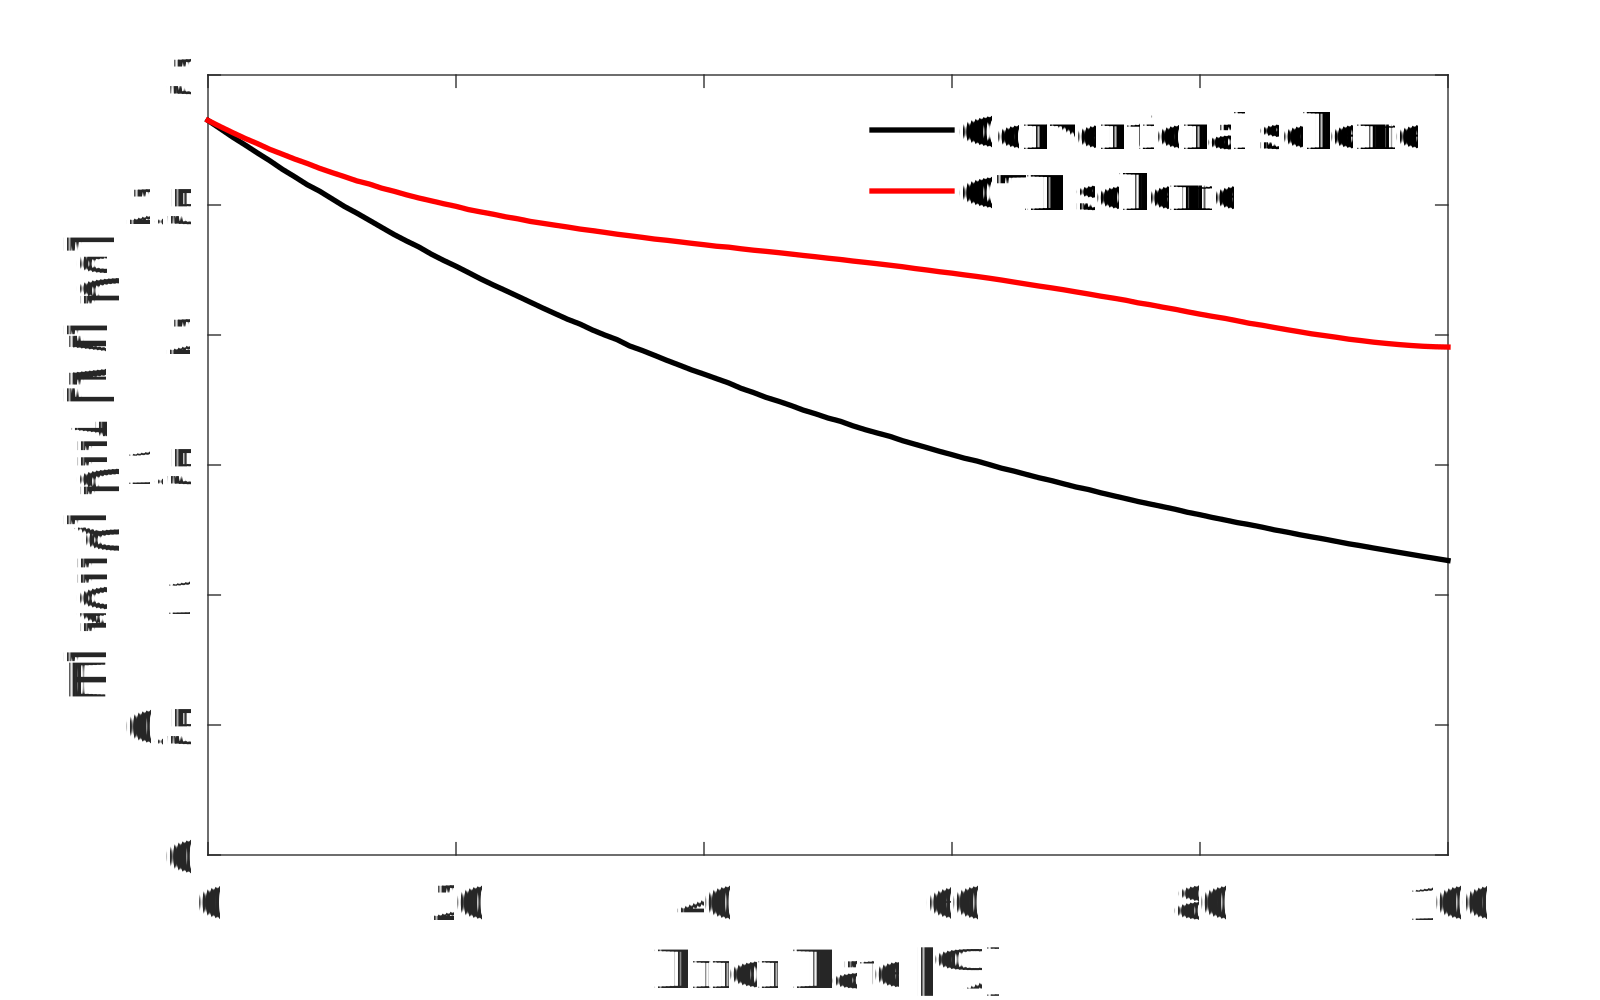
\includegraphics[width=\linewidth]{throughput_probabilistic_retry_v3.pdf} % 図のファイル名を指定
  \caption{誤り率に対するスループット特性}
  \label{fig:throughput_v3} % 参照用ラベル
\end{figure}
\begin{figure}[H]
  \centering
  \includegraphics[width=\linewidth]{throughput_probabilistic_retry_v3.1.pdf} % 図のファイル名を指定
  \caption{誤り率に対する総送信回数の変化}
  \label{fig:throughput_v3.1} % 参照用ラベル
\end{figure}

\section{まとめ}
本稿では,直線に配置されたドローン中継伝送におけるオーバリーチ干渉の影響を解決するために,送信信号の届く中継局まで一回で中継するCTR方式を検討した.
CTR方式と従来の方式で誤りが生じたときとそうでないときのスループット特性を計算し比較した.
この結果からいずれの条件でもCTR方式が従来方式よりも高いスループットが得られることを確認した.

\begin{thebibliography}{99}
  \bibitem{ref1}設樂,他,“ドローンの直線中継伝送におけるアクセス制御方式の一検討,” 電子情報通信学会大会講演論文 B‐11‐2,2018年9月
\end{thebibliography}

% ---------
% 文献リスト
% ---------
%\bibliography{arxiv} % bibファイルを指定 (例: arxiv.bib)
%\bibliographystyle{junsrt}

\end{document}
